\section{实验九:File system}\label{sec:File_system}

\subsection{实验目的}

\begin{enumerate}
	\item 理解 UNIX 系统以及 xv6 系统组织文件的方式,包括 inode 数据结构以及地址的映射关系。
	\item 掌握通过增加索引级数的文索引扩展方式。
	\item 理解文件映射和打开的方式,了解 xv6 系统的文件系统层级架构。
	\item 理解硬链接和软链接的实现方式。
\end{enumerate}

\subsection{实验准备}

\subsubsection{文件系统概述}

xv6 的文件系统一共有七层,如\cref{fig:file_layers} 所示,每一层的作用如下:

\begin{enumerate}
	\item disk 磁盘层:对 virtio 硬盘上的文件块进行读写操作。z
	\item buffer cache 高速缓存层:对磁盘文件块进行缓存,并确保只有1个内核进程能在一段时间内修改文件块上存储的数据。
	\item logging 日志层:让更高的层级能够将对文件块的所有 update 打包到一个 transaction 中,从而能保证所有文件块能够在将要崩溃时原子地进行update。
	\item inode 索引节点层:为每个文件提供一个独一无二的 inode number。
	\item directory 目录层:将每个文件夹作为一个特殊的 inode,这个 inode 的内容是文件夹入口。
	\item pathname 路径名层:将文件夹组织为层级,并通过递归查找来解析路径。
	\item file descriptor 文件描述符层:将管道、设备等 UNIX 资源用文件系统进行抽象。
\end{enumerate}

\begin{figure}[!htb]
	\centering
	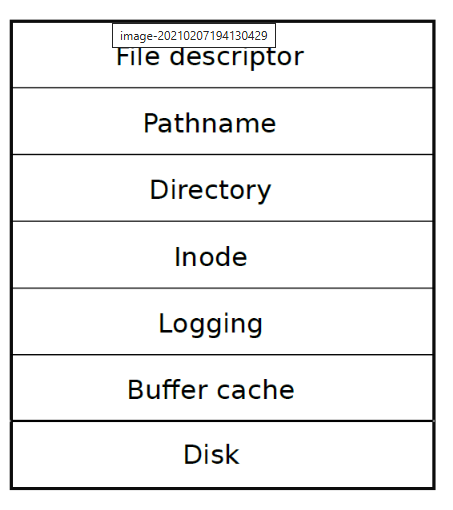
\includegraphics[width=0.4\textwidth]{file_layers}
	\caption{xv6 文件系统层级}
	\label{fig:file_layers}
\end{figure}

\subsubsection{磁盘层}

文件系统将磁盘分为了几个部分,每个部分的最小单元是 block,一个 block 的大小为 1024 字节,具体结构如\cref{fig:disk} 所示。

\begin{enumerate}
	\item block 0: 启动区域,文件系统不会使用,包含了操作系统启动所需要的代码
	\item blcok 1: 超级块,存储了文件系统的元数据(块的大小、块的数目、索引节点数、日志中的块数),里面有一个 mkfs 的程序,用来构建初始的文件系统。
	\item block 2-31:日志块:用于保存日志。
	\item block 32-44: 索引节点块,一个 inode 的大小为 64 字节,一个 block 的大小为 1024 字节,因此 block32 为inode 1-16,block33 为 inode 17-32。
	\item block 45 :位图块,用来跟踪哪些块在使用。
    \item block 46 以及后:数据块,要么是在位图中中被标记为空闲状态,要么存储了文件/文件夹的内容。
\end{enumerate}

\begin{figure}[!htb]
	\centering
	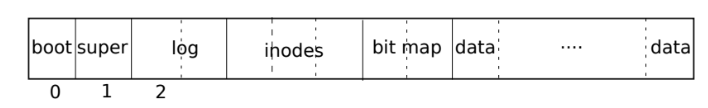
\includegraphics[width=0.6\textwidth]{disk}
	\caption{xv6 文件系统结构}
	\label{fig:disk}
\end{figure}

\subsubsection{高速缓存层}

高速缓存层有两个作用:

\begin{enumerate}
	\item 将对磁盘块的访问权限进行同步,保证内存中只保存一个该磁盘块的拷贝,且一次只有一个内核线程访问这个拷贝,但同时可以有多个对这个 block 的引用。
	\item 将被频繁访问的块缓存到内存中。
\end{enumerate}

高速缓存(\texttt{bcache} 结构体)中的 \texttt{buf} 数量为 \texttt{NBUF},因此当新的文件块需要加入缓冲区时,需要将最早使用的缓冲区中的文件块替换为新的文件块。缓冲区的使用早晚通过 \texttt{head} 来判断。

buffer cache 本身是一个双向链接的链表,链表元素为 buf 结构体。其定义和初始化如\cref{lst:buf_and_binit} 所示。

\begin{listing}[!htb]
	\begin{minted}{c}
struct buf {
    int valid;   // has data been read from disk?
    int disk;    // does disk "own" buf?
    uint dev;
    uint blockno;
    struct sleeplock lock;
    uint refcnt;
    struct buf *prev; // LRU cache list
    struct buf *next;
    uchar data[BSIZE];
    uint timestamp;
};

struct {
    struct spinlock lock;
    struct buf buf[NBUF];
    struct buf head;
} bcache;

void
binit(void)
{
    struct buf *b;

    initlock(&bcache.lock, "bcache");

    // Create linked list of buffers
    bcache.head.prev = &bcache.head;
    bcache.head.next = &bcache.head;
    for(b = bcache.buf; b < bcache.buf+NBUF; b++){
        b->next = bcache.head.next;
        b->prev = &bcache.head;
        initsleeplock(&b->lock, "buffer");
        bcache.head.next->prev = b;
        bcache.head.next = b;
    }
}
	\end{minted}
	\caption{buf 结构体和 binit 函数}\label{lst:buf_and_binit}
\end{listing}

bguffer cache 层导出的主接口主要是 \texttt{bread} 和 \texttt{bwrite};前者获取一个 \texttt{buf},其中包含一个可以在内存中读取或修改的块的副本,后者将修改后的缓冲区写入磁盘上的相应块。内核线程必须通过调用 \texttt{brelse} 释放缓冲区。buffer cache 每个缓冲区使用一个睡眠锁,以确保每个缓冲区(因此也是每个磁盘块)每次只被一个线程使用;\texttt{bread} 返回一个上锁的缓冲区,\texttt{brelse} 释放该锁。

\subsubsection{日志层}

很多对文件系统的操作都涉及了对硬盘的多次写入,当某次写入后发生崩溃将导致文件系统出现问题。

xv6 通过日志层解决该问题。在 xv6 中,系统调用不会直接对硬盘上的块进行写入,而是将所有想要进行的对硬盘的写入操作的描述放到日志中,当系统调用将所有的写入操作都放到日志后,会向硬盘写入一个提交记录,来表示这个日志已经记录了所有的操作,然后系统调用进行全部的写入操作,并将硬盘上的日志全部清除。

当操作系统崩溃后进行重启,将在进行任何进程之前从崩溃中恢复。如果在对硬盘的所有写入操作提交之前发生了崩溃,那么这个日志将被视为不完整的,xv6 将直接忽略它,如果崩溃发生在提交之后,说明这个日志是完整的,则恢复系统将重复这些步骤,最后删除日志。在任何一种情况下,日志都会使操作在崩溃时成为原子操作:恢复后,要么操作的所有写入都显示在磁盘上,要么都不显示。

\subsubsection{日志设计}

日志驻留在超级块中指定的已知固定位置。它由一个头块(header block)和一系列更新块的副本(logged block)组成。头块包含一个扇区号数组(每个logged block对应一个扇区号)以及日志块的计数,这种设计确保了日志的可定位性和完整性。

磁盘上的头块中的计数或者为零,表示日志中没有事务;或者为非零,表示日志包含一个完整的已提交事务,并具有指定数量的 logged block。因此,事务中途崩溃将导致日志头块中的计数为零;提交后的崩溃将导致非零计数。这种设计使得系统能够准确判断崩溃发生时事务的状态,从而决定是否需要执行恢复操作,确保崩溃恢复的准确性。

每个系统调用的代码都指示写入序列的起止,考虑到崩溃,写入序列必须具有原子性。为了允许不同进程并发执行文件系统操作,日志系统可以将多个系统调用的写入累积到一个事务中,这种设计既保证了原子性又提高了并发性。同时提交多个事务的想法称为组提交(group commit)。组提交减少了磁盘操作的数量,因为成本固定的一次提交分摊了多个操作。组提交还同时为磁盘系统提供更多并发写操作,可能允许磁盘在一个磁盘旋转时间内写入所有这些操作,显著提高了系统性能。

Xv6 在磁盘上留出固定的空间来保存日志。事务中系统调用写入的块总数必须可容纳于该空间。这导致两个后果:任何单个系统调用都不允许写入超过日志空间的不同块,这对大多数系统调用来说都不是问题,但其中两个可能会写入许多块:write和unlink。一个大文件的 \texttt{write} 可以写入多个数据块和多个位图块以及一个 \texttt{inode} 块;\texttt{unlink} 大文件可能会写入许多位图块和 \texttt{inode}。Xv6 的 \texttt{write} 系统调用将大的写入分解为适合日志的多个较小的写入,\texttt{unlink} 不会导致此问题,因为实际上 Xv6 文件系统只使用一个位图块。

\subsubsection{索引节点层}

inode(即索引结点)可以具有两种相关含义之一。它可能是指包含文件大小和数据块编号列表的磁盘上的数据结构,或者指内存中的索引节点,它包含磁盘上索引节点的副本以及内核中所需的额外信息。

磁盘上的 inode 放在一个连续的区域内,这个区域有很多 block,叫做 inode block,每个 inode 大小相同,为 64 字节,由 \texttt{truct dinode} 定义,如\cref{lst:dinode} 所示。字段 \texttt{type} 为零表示磁盘 \texttt{inode} 是空闲的。字段 \texttt{nlink} 统计引用此 \texttt{inode} 的目录条目数,以便识别何时应释放磁盘上的 \texttt{inode} 及其数据块。字段 \texttt{size} 记录文件中内容的字节数。 \texttt{addrs} 数组记录保存文件内容的磁盘块的块号。


\begin{listing}[!htb]
	\begin{minted}{c}
struct dinode {
    short type;           // File type
    short major;          // Major device number (T_DEVICE only)
    short minor;          // Minor device number (T_DEVICE only)
    short nlink;          // Number of links to inode in file system
    uint size;            // Size of file (bytes)
    uint addrs[NDIRECT+1];   // Data block addresses
};
	\end{minted}
	\caption{dinode 结构体的定义}\label{lst:dinode}
\end{listing}


内存中的 inode 是 active inodes,用struct inode定义,如\cref{lst:inode} 所示。active inodes 指内存中有指针指向这个 inode,\texttt{ref} 字段统计引用内存中 \texttt{inode} 的 \texttt{C} 指针的数量,如果引用计数降至零,内核将从内存中丢弃该 \texttt{inode}。 \texttt{iget} 和 \texttt{iput} 函数分别获取和释放指向 \texttt{inode} 的指针,修改引用计数。

\begin{listing}[!htb]
	\begin{minted}{c}
struct inode {
    uint dev;           // Device number
    uint inum;          // Inode number
    int ref;            // Reference count
    struct sleeplock lock; // protects everything below here
    int valid;          // inode has been read from disk?
    
    short type;         // copy of disk inode
    short major;
    short minor;
    short nlink;
    uint size;
    uint addrs[NDIRECT+1];
};
	\end{minted}
	\caption{inode 结构体的定义}\label{lst:inode}
\end{listing}

inode 层一共有四种锁:

\begin{enumerate}
	\item \texttt{icache.lock} 负责确保 1 个 \texttt{inode} 只在 \texttt{cache} 中出现最多 1 次,并且保证 \texttt{ref} 正确记录引用到这个 \texttt{inode} 的数量,因此对 \texttt{ref} 的修改都需要用 \texttt{icache.lock} 进行保护。
	\item 每个 \texttt{inode} 自己也有 1 个 \texttt{lock} 来保护对 \texttt{inode} 成员变量以及 \texttt{inode} 指向的文件或文件夹的内容的保护。
	\item \texttt{ref} 是内存中指向这个 \texttt{inode} 的个数,当 \texttt{ref} 大于 0 时,不会将这个 \texttt{inode} 从 \texttt{icache} 中剔除。
	\item \texttt{nlink} 这个成员变量在 on-disk \texttt{inode} 中也存在,统计指向这个文件的 \texttt{directory entry} 的个数,当为 0 时将释放掉这个 \texttt{inode}。
\end{enumerate}

\subsubsection{目录层}

目录和文件的实现类似,它的 \texttt{inode} 类型为 \texttt{T\_DIR},其数据是一系列目录条目(directory entries)。每个条目( \texttt{entry})都是一个 \texttt{struct dirent},如 \cref{lst:dirent} 所示,其中包含一个名称 \texttt{name} 和一个 \texttt{inode} 编号 \texttt{inum}。名称最多为 \texttt{DIRSIZ}(14)个字符;如果较短,则以 \texttt{NULL}(0)字节终止。 \texttt{inode} 编号为零的条目是空的。

\begin{listing}[!htb]
	\begin{minted}{c}
struct dirent {
    ushort inum;
    char name[DIRSIZ];
};
	\end{minted}
	\caption{dirent 结构体的定义}\label{lst:dirent}
\end{listing}

函数 \texttt{dirlookup} 在目录中搜索具有给定名称的条目。如果找到,它将返回一个指向相应 \texttt{inode} 的指针,解开锁定,并将 \texttt{poff} 设置为目录中条目的字节偏移量,以满足调用方希望对其进行编辑的情形。

\texttt{dirlookup} 是 \texttt{iget} 没有直接对 \texttt{inode} 上锁的原因,因为在调用 \texttt{dirlookup} 的时候,实际上已经对 \texttt{dp} 上锁了,如果查找的 \texttt{directory entry} 是 \texttt{.}(当前文件夹/ \texttt{inode} 本身),那么会试图对 \texttt{dp} 再 \texttt{acquire} 一次锁,造成死锁。

函数 \texttt{dirlink} 将给定名称和 \texttt{inode} 编号的新目录条目写入目录 \texttt{dp}。如果名称已经存在, \texttt{dirlink} 将返回一个错误。主循环读取目录条目,查找 \texttt{dp} 中尚未分配的 \texttt{entry}( \texttt{inum==0}),如果找到了就将 \texttt{off} 设置为这个 \texttt{entry} 的 \texttt{offset},然后用 \texttt{writei} 写入,如果没有找到就将 \texttt{off} 设置为 \texttt{dp->size},将这个 \texttt{entry} 加在最后。

\subsubsection{路径名层}

路径名查找涉及一系列对 \texttt{dirlookup} 的调用,每个路径组件调用一个。
\texttt{namei} 函数负责对路径名进行解析,并返回 \texttt{inode}。 

\texttt{namei} 调用了 \texttt{namex} 函数, \texttt{namex} 中传入了参数 \texttt{nameiparent},当为 1 时返回的 inode 是传入 path 的父文件夹,并将最后的 element 名称复制到 \texttt{name} 中。 \texttt{namex} 不断调用了 \texttt{skipelem},一步步将当前的 \texttt{inode} 变为下一级 \texttt{inode},直到得到最终需要的 \texttt{inode} 为止。注意:在每个循环中都要先进行 \texttt{ilock(ip)},因为直到 \texttt{ilock} 才能保证 \texttt{ip->type} 从硬盘中读取。

由于 \texttt{namex} 中可能涉及到多个 data block 的 I/O,因此可能是比较耗时的,当一个 kernel thread 执行 \texttt{namex} 被 disk I/O 阻塞时,其他 thread 再执行 \texttt{namex} 查找不同的文件夹 path 时不会被阻塞。

\subsubsection{文件名描述符层}

文件名描述符层(file descriptor layer)可以让 UNIX 中的所有资源,包括设备(比如console)来统一表示为文件。每个打开的文件(file descriptor)都用 \texttt{struct file} 来表示,这是一个 pipe/inode/device 的包装结构体,如\cref{lst:file} 所示。

\begin{listing}[!htb]
	\begin{minted}{c}
struct file {
    enum { FD_NONE, FD_PIPE, FD_INODE, FD_DEVICE } type;
    int ref; // reference count
    char readable;
    char writable;
    struct pipe *pipe; // FD_PIPE
    struct inode *ip;  // FD_INODE and FD_DEVICE
    uint off;          // FD_INODE
    short major;       // FD_DEVICE
};
	\end{minted}
	\caption{file 结构体的定义}\label{lst:file}
\end{listing}

system call 调用一次 \texttt{open()} 将增加一个新的打开文件(一个新的 \texttt{struct file}),同一个 \texttt{file} 可以被多个不同的进程 \texttt{open},出现在这些进程的文件表中。 \texttt{struct file} 中的 reference count 记录了同一个文件被引用的次数。

所有打开的文件都保存在全局文件表 \texttt{ftable} 中。
\texttt{filealloc} 负责在 \texttt{file table} 中分配一个文件,在 \texttt{ftable} 中扫描 \texttt{ref==0} 的 \texttt{file},增加 \texttt{ref} 后返回这个 \texttt{file}。

\texttt{filedup} 负责对这个 \texttt{file descriptor} 的 \texttt{ref++} 并返回这个文件的 \texttt{file}。

\texttt{fileclose} 负责对 \texttt{file descriptor} 的 \texttt{ref--},当 \texttt{ref==0} 时根据这个 \texttt{file} 的类型释放掉 \texttt{pipe} 或者 \texttt{inode}。

\texttt{fileread} 和 \texttt{filewrite} 分别确认 \texttt{f->readable} 和 \texttt{f->writable} 是否允许当前的读写操作,然后再根据 \texttt{f->type} 是 \texttt{FD\_PIPE/FD\_DEVICE/FD\_INODE} 进行对应的 \texttt{piperead/readi} 等操作。 \texttt{fileread} 和 \texttt{filewrite} 都使用了 \texttt{f->off} 来指示当前的读写到了哪一个位置。

\subsection{实验内容}

\begin{enumerate}
	\item 修改文件系统使其支持更大的文件存储。具体做法是实现二级间接的索引节点(inode)。
	\item 增加一个通过符号链接的系统调用。将目标符号与系统路径链接,使对符号文件的操作都同步到对相应路径文件的操作。
\end{enumerate}

\subsection{实验过程}

\subsubsection{实现 Large files}

修改 xv6 文件系统代码,使其支持每个 inode 中的“双重间接”块,其中包含 256 个单间接块地址,每个单间接块最多可包含 256 个数据块地址。这样,一个文件最多可以包含 65803 个块,即 256*256+256+11 个块(11 个而不是 12 个,因为我们将为双重间接块牺牲一个直接块编号)。

\begin{enumerate}
	\item 在 kernel/fs.h 中修改相关宏定义,如\cref{lst:modify_fs} 所示。
	\item 由于 \texttt{NDIRECT} 改变,其中一个直接快变成了二级间接块,需要修改 inode 中 \texttt{addrs} 元素的数量,如\cref{lst:modify_inode_addr} 所示。
	\item 修改 \texttt{bmap},使其支持二级索引,如\cref{lst:bmap} 所示。
	\item 修改 \texttt{itrunc},使其释放所有块,如\cref{lst:itrunc} 所示。
	\item 在 qemu 中输入 bigfile,通过测试,如\cref{fig:test_bigfile} 所示。
\end{enumerate}

\begin{listing}[!htb]
	\begin{minted}{c}
#define NDIRECT 11
#define NINDIRECT (BSIZE / sizeof(uint))
#define NININDIRECT (BSIZE / sizeof(uint)) * (BSIZE / sizeof(uint))
#define MAXFILE (NDIRECT + NINDIRECT + NININDIRECT)
#define NADDR_PER_BLOCK (BSIZE / sizeof(uint))  // 一个块中的地址数量
	\end{minted}
	\caption{修改 fs.h 相关宏定义}\label{lst:modify_fs}
\end{listing}

\begin{listing}[!htb]
	\begin{minted}{c}
// fs.h
struct dinode {
    ...
    uint addrs[NDIRECT + 2];   // Data block addresses
};

// file.h
struct inode {
    ...
    uint addrs[NDIRECT + 2];
};

	\end{minted}
	\caption{修改 inode 中 addrs 元素}\label{lst:modify_inode_addr}
\end{listing}

\begin{listing}[!htb]
	\begin{minted}{c}
static uint
bmap(struct inode *ip, uint bn)
{
    uint addr, *a;
    struct buf *bp;
    
    if(bn < NDIRECT){
        ...
    }
    
    bn -= NDIRECT;
    
    if(bn < NINDIRECT){
        ...
    }
    
    bn -= NINDIRECT;

    if(bn < NININDIRECT){
        uint addr1 = bn / NADDR_PER_BLOCK;
        uint addr2 = bn % NADDR_PER_BLOCK;
        
        // 获取双重间接块
        uint double_indirect_block;
        if((double_indirect_block = ip->addrs[NDIRECT+1]) == 0){
            double_indirect_block = ip->addrs[NDIRECT+1] = balloc(ip->dev);
        }
        
        // 读取双重间接块
        bp = bread(ip->dev, double_indirect_block);
        a = (uint*)bp->data;
        
        // 获取单间接块号
        uint single_indirect_block;
        if((single_indirect_block = a[addr1]) == 0){
            single_indirect_block = a[addr1] = balloc(ip->dev);
            log_write(bp);
        }
        brelse(bp);
        
        // 读取单间接块
        bp = bread(ip->dev, single_indirect_block);
        a = (uint*)bp->data;
        
        // 获取数据块号
        uint data_block;
        if((data_block = a[addr2]) == 0){
            data_block = a[addr2] = balloc(ip->dev);
            log_write(bp);
        }
        brelse(bp);
        return data_block;
    }
    panic("bmap: out of range");
}
	\end{minted}
	\caption{修改 bmap 使其支持二级索引}\label{lst:bmap}
\end{listing}

\begin{listing}[!htb]
	\begin{minted}{c}
void
itrunc(struct inode *ip)
{
    int i, j;
    struct buf *bp;
    uint *a;
    
    for(i = 0; i < NDIRECT; i++){
        ...
    }
    
    if(ip->addrs[NDIRECT]){
        ...
    }
    
    struct buf *bp1;
    uint *a1;
    if(ip->addrs[NDIRECT+1]){
        bp = bread(ip->dev, ip->addrs[NDIRECT+1]);
        a = (uint*)bp->data;
        for(i = 0;i < NADDR_PER_BLOCK; i++){
            if(a[i]){
                bp1 = bread(ip->dev, a[i]);
                a1 = (uint*)bp1->data;
                
                for(j = 0;j<NADDR_PER_BLOCK; j++){
                    if(a1[j])
                    bfree(ip->dev, a1[j]);
                }
                
                brelse(bp1);
                bfree(ip->dev, a[i]);
            }
        }
        brelse(bp);
        bfree(ip->dev, ip->addrs[NDIRECT+1]);
        ip->addrs[NDIRECT+1] = 0;
    }
    ip->size = 0;
    iupdate(ip);
}
	\end{minted}
	\caption{修改 itrunc 释放所有块}\label{lst:itrunc}
\end{listing}

\begin{figure}[!htb]
	\centering
	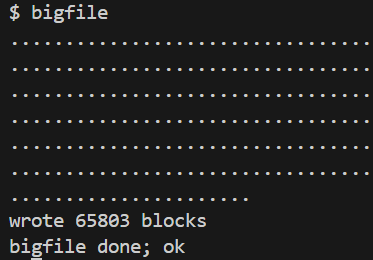
\includegraphics[width=0.5\textwidth]{test_bigfile}
	\caption{测试 bigfile}
	\label{fig:test_bigfile}
\end{figure}

\subsubsection{实现 Symbolic links}

\begin{enumerate}
	\item 为 symlink 创建一个新的系统调用号,在 user/usys.pl、user/user.h 中添加一个条目,,在 kernel/syscall.c、kernel/syscall.h 中添加相关内容,并在  kernel/sysfile.c 中实现一个空的 sys\_symlink。
	\item 添加提示中的相关定义 \texttt{T\_SYMLINK} 以及\texttt{O\_NOFOLLOW},如\cref{lst:add_define}。
	\item 实现 \texttt{sys\_symlink},使用 \texttt{create} 返回已加锁的 inode,\texttt{iunlockput} 既对 inode 解锁,还将其引用计数减 1,计数为 0 时回收此 inode,如\cref{lst:sys_symlink} 所示。
	\item 修改 \texttt{sys\_open} 使其支持打开符号链接,如\cref{lst:sys_open} 所示。
	\item 在 qemu 中输入 symlinktest 和 usertests,通过测试,如\cref{fig:test_symlink} 和\cref{fig:test_usertests} 所示。
\end{enumerate}

\begin{listing}[!htb]
	\begin{minted}{c}
// fcntl.h
#define O_NOFOLLOW 0x004

// stat.h
#define T_SYMLINK 4
	\end{minted}
	\caption{添加相关宏定义}\label{lst:add_define}
\end{listing}

\begin{listing}[!htb]
	\begin{minted}{c}
uint64
sys_symlink(void){
    char target[MAXPATH],path[MAXPATH];
    struct inode *ip;
    if(argstr(0, target, MAXPATH) < 0 || argstr(1, path, MAXPATH) < 0)
        return -1;
    
    if(strlen(target) > MAXPATH)
        return -1;
    
    begin_op();
    ip = create(path,T_SYMLINK,0,0);
    
    if(ip == 0){
        end_op();
        return -1;
    }
    
    if(writei(ip,0,(uint64)target,0,strlen(target))!=strlen(target)){
        iunlockput(ip);
        end_op();
        return -1;
    }
    
    iunlockput(ip);
    end_op();
    return 0;
}
		
	\end{minted}
	\caption{实现 sys\_symlink}\label{lst:sys_symlink}
\end{listing}

\begin{listing}[!htb]
	\begin{minted}{c}
uint64
sys_open(void)
{
    char path[MAXPATH];
    int fd, omode;
    struct file *f;
    struct inode *ip;
    int n;

    ...	
    
    if(ip->type == T_DEVICE && (ip->major < 0 || ip->major >= NDEV)){
        ...
    }
    
    if(ip->type == T_SYMLINK && !(omode & O_NOFOLLOW)){
        for(int i = 0; i < 10; i++){
            if(readi(ip,0,(uint64)path,0,MAXPATH-1) <= 0){
                iunlockput(ip);
                end_op();
			    return -1;
			}
            path[n] = '\0';
            
            iunlockput(ip);
            if((ip = namei(path)) == 0){
                end_op();
                return -1;
            }
            
            ilock(ip);
            if(ip->type!=T_SYMLINK)
                break;
        }
        if(ip->type == T_SYMLINK){
            iunlockput(ip);
            end_op();
		    return -1;
        }
    }
    
    if((f = filealloc()) == 0 || (fd = fdalloc(f)) < 0){
        ...
    }
    
    ...
   
    return fd;
}		
	\end{minted}
	\caption{实现 sys\_open}\label{lst:sys_open}
\end{listing}

\begin{figure}[!htb]
	\centering
	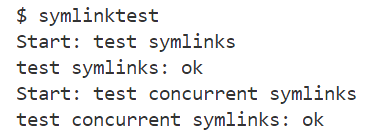
\includegraphics[width=0.5\textwidth]{test_symlink}
	\caption{测试 symlink}
	\label{fig:test_symlink}
\end{figure}

\begin{figure}[!htb]
	\centering
	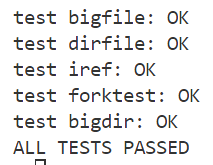
\includegraphics[width=0.5\textwidth]{test_usertests}
	\caption{测试 usertests}
	\label{fig:test_usertests}
\end{figure}

\subsubsection{综合测试}

在 xv6-labs-2021 目录下创建一个 time.txt文件,记录该lab花费的时间。使用 \texttt{make grade} 对 lab9 进行综合测试,测试通过。

\begin{figure}[!htb]
	\centering
	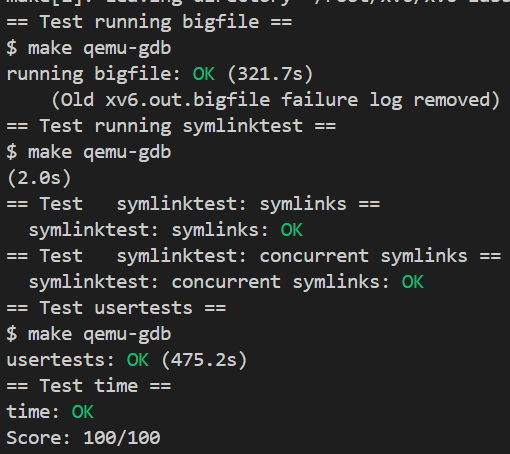
\includegraphics[width=0.5\textwidth]{test_lab9}
	\caption{测试 lab9}
	\label{fig:test_lab9}
\end{figure}

\subsection{实验小结}

本次试验是关于 xv6 系统文件系统的,拓展了可以索引的文件大小,也创建了符号链接这种软链接方式。

第一个部分中的拓展文件大小是一个典型的程序数据结构设计思想,可以看作是对于一个高度为 1 的树,将其某一些节点拓展成指向相似的节点的非叶子结点,从而扩展这个数的容量(使其高度增加)。这种思想被运用在可拓展地址数的操作数设计(计算机组成原理课程中),以及多级页表的设计(操作系统课程中)。实现这一功能的过程十分有趣。

第二个部分是实现系统文件软链接相关的内容。这个部分在课程内要求不高, 在实现的过程中最大的困难在于理解“软链接也是一种文件”这一概念。这个实 验让我加深了对电脑上那些左下角有箭头符号的文件本质是什么这一问题理解。
